\documentclass{article}
\usepackage[utf8]{inputenc}
\usepackage{fullpage}

%Tables
\usepackage{multirow}
\usepackage[table]{xcolor}
\definecolor{blue}{HTML}{4E60F0}

%Math
\usepackage{amssymb, stmaryrd}
\usepackage[fleqn]{amsmath}

%Graphics
\usepackage{graphicx}
\graphicspath{{./fig/}}
\usepackage{subcaption}

%Comments
%MORA
\newcommand{\changeMM}[2]{{\leavevmode\color{red}{\scriptsize\st{#1}}~\color{red}#2}}
\newcommand{\nbMM}[1]{{\leavevmode\color{red}{\scriptsize#1}}}
\newcommand{\addMM}[1]{{\leavevmode\color{red}#1}}

%EWAN
\newcommand{\changeED}[2]{{\leavevmode\color{blue}{\scriptsize\st{#1}}~\color{blue}#2}}
\newcommand{\nbED}[1]{{\leavevmode\color{blue}{\scriptsize#1}}}
\newcommand{\addED}[1]{{\leavevmode\color{blue}#1}}

%EMMANUEL
\newcommand{\changeEC}[2]{{\leavevmode\color{green}{\scriptsize\st{#1}}~\color{green}#2}}
\newcommand{\nbEC}[1]{{\leavevmode\color{green}{\scriptsize#1}}}
\newcommand{\addEC}[1]{{\leavevmode\color{green}#1}}

\title{LDA for Mouse Tracking}

\begin{document}
\maketitle

\section{Background}

\begin{itemize}

\item Mouse-tracking has proved to be an useful measurement of the processes underlying decision making in different domains, ranging from phonetic competition (Spivey, Grosjean, \& Knoblich, 2005), and syntactic and pragmatic processing (Farmer, Anderson, \& Spivey, 2007; Tomlinson, Bailey, \& Bott, 2013) to social cognition (Freeman \& Ambady, 2010; Freeman, Dale, \& Farmer, 2011). 

\item In particular, mouse tracking has initially served to disentangle between serial and parallel accounts for a single cognitive process: Whenever processing involves two independent and subsequent processes \addMM{(what we could call a ``change of decision")}, mouse trajectories are expected to be displayed as two movements (i.e. with a change of trajectory); whereas dynamic/parallel accounts would predict a single smooth and graded movement (Wojnowicz et al., 2009).  

\item The reliability of mouse tracking resides in the fact that motor responses seem to be prepared in parallel to the decision and performed in a cascade manner (i.e., as fast as they can be executed) (Song \& Nakayama, 2006; Freeman \& Ambady, 2010). Therefore, just as eye movements (Rayner, 1998; Just et al., 1982)\footnote{The main advantage of mouse tracking over eye tracking is the simplicity of the set up, which can be even tested online.}, mouse paths might reveal decision dynamics with fine-grained temporal resolution (Freeman et al., 2011; Freeman \& Ambady, 2010; Hehman, Stolier, \& Freeman, 2014).  

\item Basic paradigm

\begin{itemize}

\item The standard task used to test with a mouse tracking paradigm is a two-alternative forced choice where participants are presented with a stimulus and then they have to make a choice using the options appearing in the top left or right corner. In each trial, participants have to press a “Start” button, located at the middle bottom of the screen, to see the stimulus. As participants move the mouse cursor to select the response, x,y coordinates are recorded. 

\item A software package called MouseTracker has been developed but the same can be done using standard programming techniques. In what follows, we will present results obtained for a online experiment programmed with JavaScript. 

\end{itemize}

\begin{figure}[h]
\caption{Example Basic MT paradigm}
\end{figure}

\item In specific case of linguistics, decision dynamics can be thought as a reflection of sentence (or lexical) processing itself. Deviation towards the alternative response implies consideration of an abstract representation compatible with the response. 

\end{itemize}

\subsection{Dale and Duran 2011: Case study}

\begin{itemize}
\item Dale and Duran (2011) compared the processing of negative and affirmative sentences to test the hypothesis that negation is an operator that reverses the truth conditions of the sentence and therefore underlies an “second-step" in the derivation. 

\item The authors combined a mouse-tracking parading with a Truth Judgment Task: participants had to decide whether a general statement (e.g. cars have (no) wings) was true or false by clicking on two response buttons located at the top left and right corners.

\item The general idea behind the paradigm was that the form of the trajectory to the correct response could indicate whether participants were confident with their initial decision, whether they oscillated between the two responses (i.e. they were uncertain), or whether they considered the alternative option before ultimately select the other (i.e. whether they changed their minds). 

\item Dale and Duran computed the amount of flips on the x-coordinate (X-flips) and on the acceleration component over time. Their results suggest that mouse trajectories for affirmative sentences had less flips of both kinds than trajectories for negative sentences. Given that mouse trajectories for negative sentences were less straightforward than for affirmative sentences, they concluded that the derivation of the negative meaning was always done in a two-step manner where the affirmative meaning was initially derived and negated afterwards.    

\end{itemize}

\subsection{Top 5 measures to test changes of decision}
%Mention potential confounds in the interpretation of these measures
A full review is provided in Hehman et al. (2014). Here, we would just discuss the 5 measures that have been more extensively used. 

\begin{itemize}


\item \textbf{Spatial analyses.} Typically rely on the x,y coordinates themselves and their distance to each of the possible responses (target response and alternative response). They evaluate the degree of unpredictability and complexity of the path. 

\begin{itemize}
\item \textit{Area under the curve}: Geometric area between the observed mouse-trajectory and an idealised straight-line trajectory drawn from the start and end point. Higher values are associated with higher deviation peaks towards the alternative; values closer to zero (or below) suggest trajectory close to ideal. \\ 
AUC \(= \sum (\Delta x_{t} - \Delta x_{t-1})(\Delta y_{t} + \Delta y_{t-1})/2  - \text{AUC}_{\text{ideal trajectory}} \)





\item \textit{Maximal deviation point}
\\ The point that maximizes the distance between the path and the ideal trajectory.  

\item \textit{X flips} (measure taken from Dale and Duran 2011)
\\``count-based score of the number of times the mouse cursor goes back and forth along the x-axis"

x-flips  \(= \sum H[(\Delta x_{t} - \Delta x_{t-1})(\Delta x_{t-1} - \Delta x_{t-2})] \)

\end{itemize}
Note that: 
\\ (a) these three options fail to distinguish between `two-step' and `uncertain' paths --i.e., trajectories with a true deviation to the alternative side or centred on the middle of the screen (\addMM{maybe put an example}). \\
(b) they are not sensitive to the moment in which the deviation peak occurs. For instance, a late deviation towards the alternative might be more strongly associated to a two-step deviation than an initial deviation towards the alternative (which could be considered just noise).

\begin{itemize}
\item \textit{Ratio of the target distance to the alternative distance} (Target:Alternative) 
\\ It compares the the distances to each response at each position. While ratio values closer to 1 suggest a position near the middle, higher values indicate a deviation towards the alternative response.  
\\Ratio values can be analyzed in two alternative ways, either by extracting their maximum -- the point that maximizes the ratio between distances-- or by summing the values in time -- area under ratio curve. In the former case, erratic changes of the path (averaged in zero) will be dissociated from real "two-step" decisions. 
\end{itemize}

\item \textbf{Speed and acceleration.} Temporal measurements analyze the dynamics of the decision, addressing the degree of competition at different time steps. 
Stronger competition between alternative responses is typically translated into steeper  acceleration peaks (Hehman et al., 2014). In addition, the decision point has also been associated with temporal measures such as acceleration peak and time of highest spatial deviation, either maximum ratio or maximum deviation. Importantly, in the former case, the decision is considered to appear just after the maximal deviation/maximal ration point, whereas last acceleration peaks are typically after.

The ``acceleration component'' used on Dale and Duran 2011 (and more generally in studies on error correction) is analyzed as a function of the number of times that the trajectory accelerates/decelerates. 

Acceleration component (or Acceleration flips) \(= (\sum H[(\Delta a_{t} - \Delta a_{t-1})(\Delta a_{t-1} - \Delta a_{t-2})])-1 \)

\end{itemize}

\begin{figure}
\caption{Different spatial measurements.}
\end{figure}


\section{Goals}

\begin{itemize}
%When we talk about changing decision we are actually taking about considering first one alternative as the response and then the other one. 

\item The basic assumption of most MT studies is that, whenever a participant changes her decision, this change will be reflected somehow in the mouse trajectory. That is to say, it will have a specific signature associated, such as spatial deviation towards the alternative. From this assumption, one can conclude that a change of decision has occurred whenever the signature is present. 

\item However, the link between decision change and specific signatures is not as straightforward as one might desire. For instance, the existence of a deviation towards the alternative response has shown to be neither a necessary nor a sufficient condition for a change of decision:

\begin{itemize}
\item Not all deviated trajectories imply a change of decision.
\item Not all decision changes are reflected in a deviation in mouse trajectories.
\end{itemize}

\item In this paper, our goal is twofold:

\begin{itemize}
\item[1.] \textbf{Validate measures used to check decision change.} 
Instead of concluding a change of decision from fluctuations in one particular measure, we will explicitly manipulate whether there is or not a change of decision. We reason that trajectories for trials that involve a change of decision should all share meaningful components. Therefore, we can test which of the measures is the one that maximizes the difference between trajectories that underly a change of decision and the ones that do not.

\item[2.] \textbf{Present a new measure to check decision change, based on a classifier.} We will use the validation data (cf. 1 above) to train a \emph{linear discriminant analysis} (henceforth, LDA). The LDA will classify trajectories into the ones that underly a change of decision and the ones that do not. Once the classifier is trained, we will test it with new data, obtained from a replication of Dale and Duran (2011).   

Unlike most measures mentioned above, the LDA has the advantage that it also allows for a three-way categorization: we could also make a second distinction between trajectories classified as ``not-change", between the ones that underly uncertainty and the ones that underly a rapid decision. 

\end{itemize}

\item Note, moreover, that given that our experiments were performed online, we can ensure that the measure is somehow resistant to noisy data.

\end{itemize}

\section{Training the classifier}

\subsection{The classifier: Linear discriminant analysis}
\begin{itemize}
\item LDA: linear method for classification (decision boundary between two or more classes). Assuming the different classes have a common covariance matrix, the classifier tries to find a linear combination of predictors that gives maximum separation between the classes. 
% Model the distribution of predictors given the class and use Bayes' theorem to flip these into P(class|predictor). 

\item The linear coefficient provides the linear combination of predictors used to form the decision rule. 

\item Which features should the classifier take as predictors? \addMM{(to apply the PCA and then the LDA)}\\
Testing the classifier with different sources of information can give us information about which features of the mouse trajectory are more relevant for the distinction. We train and test the classifier with different combinations of three features:

\begin{itemize}
\item x,y Coordinates. 

\item Velocity and Acceleration: Velocity is calculated as the distance between subsequent coordinates at different time points, and acceleration may be computed from changes in velocity across time points. 
These values can be computed on the basis of (a) each coordinate: x-coordinates only (horizontal velocity/acceleration) and y-coordinates only (vertical velocity/acceleration), or (b) both coordinates (Euclidean-based velocity/acceleration). 

\item LogRatio: For each x,y coordinate (position), we calculate the ratio between the euclidean distance to the alternative response and the distance to the target response. This value was log transformed. 
\end{itemize}


\item How do we obtain the \emph{LDA measure}? \nbMM{MM: I need to review this with Ewan. There are some steps for which I am not sure.} 
\begin{enumerate}
\item Remove dimensions that are constant between groups (coordinates that don’t change) and correlated dimensions between groups. 
\item Identify the 13 principal components on the data (PCA). 
\item Perform a LDA (linear discriminant analysis): Linear combination of the 13 PCA (predictors) that gives maximal separation between \emph{Decision change} and \emph{No decision change} classes.
\item Extract the bias: bias = $mean \ (\text{LDA/PC}_{1\times 13} \ast \text{PC/trial}_{13\times n})$
\item Obtain the \emph{LDA measure} per trial by calculating the dot product of the linear coefficients for each PC ($1\times13$ matrix) and the each PC for trial ($13 \times n$ matrix) minus the bias. \\
LDA measure = \( \text{LDA/PC}_{1\times 13} \ast \text{PC/trial}_{13\times n} -  mean \ (\text{LDA/PC}_{1\times 13} \ast \text{PC/trial}_{13\times n}) \)

\end{enumerate}


\end{itemize}

\subsection{Calibration experiment}
Participants have to perform a \emph{two-alternative forced task}: in each trial, they are presented with a colored frame surrounding the screen and they have to determinate whether the frame is blue or red. 
Responses are made by clicking on the "blue" or "red" buttons, allowing the recording of mouse-movements during each trial. Importantly, accurate responses have to describe the color at the moment of the click. In order to mimic decision processing, we manipulate whether the color of the frame remain stable along the trial or it changed at some point. 

\nbMM{MM: All this should be corrected and made specific once we run the actual calibration with the frames.}

\paragraph{Participants} N participants were recruited using Amazon Mechanical Turk. 

\paragraph{Method}

\begin{itemize}
\item There were three \textsc{Decision Type}s: (a) \textit{Straightforward}, where the decision is made at the beginning of the trial; (b) \textit{Swapped}, where the decision made at the beginning of the trial changes at some later point; and (c) \textit{Uncertain}, where the decision can only be made at a later point.  
\item The final \textsc{Frame color} (at the response moment) could be red or blue. 
\item The \textsc{Decision point} depend on the \textsc{Decision Type}. For \textit{swapped} and \textit{uncertain} trials there were three possible decision points: early, middle and late. These were determined by the y-coordinate where the color changes. 
\item The proportion was adjusted so that straightforward trials were the majority  (2/3), and people could get used to make their choice right away (without staying in the middle of the screen).
\end{itemize}

\begin{table}[!h]
\centering
\begin{tabular}{cccc}
\textsc{Decision Type}&\multicolumn{2}{c}{\textsc{Frame color}}&\textsc{Decision point}\\
\hline
\multirow{2}{*}{Straightforward} & \multicolumn{2}{c}{\cellcolor{blue} Blue} & -- \\
& \multicolumn{2}{c}{\cellcolor{red} Red} & -- \\
\hline
\multirow{2}{*}{Swapped} & \cellcolor{blue}Blue & \cellcolor{red} Red & early (y1), middle, late (y3) \\
 & \cellcolor{red} Red & \cellcolor{blue} Blue & early (y1), middle (y2), late (y3) \\
\hline
\multirow{2}{*}{Uncertain} & White & \cellcolor{red} Red & early(y1), middle, late (y3)\\
 & White & \cellcolor{blue} Blue & early (y1), middle (y2), late (y3) \\
\hline

\end{tabular}
\caption{Design in Calibration Experiment}
\end{table}

\begin{figure}
\caption{INCLUDE EXAMPLE TRIAL}
\end{figure}

\paragraph{Interface}
%The interface was programmed using JavaScript. Mouse movements triggered the extraction of x,y-pixel coordinates (i.e., no constant sample rate). The software was adapted proportionally to the window of the participant's browser, forming a rectangle: the height was covered at 100 percent and the width was 120 percent of the height. 
%Three buttons were displayed during the experiment (\textit{start} and response buttons). Their size was also determined by the browser window (i.e., approximately 20 percent of the total width). The \textit{start} box was placed at the bottom center of the screen. The two response boxes were located at the top left (\textit{blue}) and top right (\textit{red}) corners of window. This location was constant across participants, and handedness was controlled.  
%In each trial, mouse movements were recorded between start-clicks and response-clicks. The x,y-pixel trajectory was saved together with its raw time. Afterwards, the positions were normalized according to participants' window size, to allow comparisons between subjects. The normalization was done by considering the start button at the [0,0] point, the "blue" button corner at [-1,1] and the "red" button at [1,1]. 


\paragraph{Data treatment}


\begin{itemize}
\item Normalization on time by interpolation\\
Mouse-tracking data are particularly variable trial to trial. On one hand, variations in response times imply different quantity of \textit{x,y} positions per trial, making difficult the comparisons between items. On the other hand, in our design, positions are extracted based on mouse movements, and devices with more or less sensibility could influence the number of samples taken during the trial. In order to compare mouse trajectories, we normalized the time course into 101 proportional times steps (percentage of trial duration). This normalization, as all the other calculations, was performed in the Spyder environment using Python 2.7. 

\item Speed and acceleration smoothing\\
Following the procedure in Dale and Duran (2011), trajectory velocity and acceleration were computed using the distance (in pixels) covered per second over a moving window of six x,y pixel coordinates. The acceleration component was calculated after on this smoothed acceleration. 


\end{itemize}








\subsection{Performance of the classifier}

\begin{itemize}
\item Accuracy in the task
\item Mouse trajectories are sensitive to the manipulation. 
\end{itemize}

\begin{figure}
\caption{MEAN TRAJECTORIES in Calibration data}
\end{figure}


\begin{itemize}

\item Cross-validation using the Area under the (ROC) Curve

\begin{itemize}
\item The overall performance of the classifier was tested by the area under the (ROC) curve. The ROC curve will test the degree of sensitivity (percentage of change-of-mind trajectories correctly identified) and specificity (percentage of rapid-decision trajectories correctly identified) of the classifier. Given that an ideal ROC curve will hug the top left corner, the larger the AUC the better the classifier. 

\item In order to perform the ROC curve, we performed a cross validation where we partitionate the calibration data into 10 bins keeping the proportion of straight and deviated trajectories constant across bins. For each bin, we took the complementary set of data (the rest 90\%) to use as training set (to train the classifier) and use the data contained in the bin as the test set to validate the classifier. In other words, we obtained the ROC and the AUC for each bin (n=10). 
\end{itemize}

\item[(A)] LDA with different predictors

\begin{itemize}
\item Means and Distributions
\item Correlation matrix
\item AUC of ROC

\end{itemize}

\begin{figure}[h]
\begin{subfigure}{0.3\textwidth}
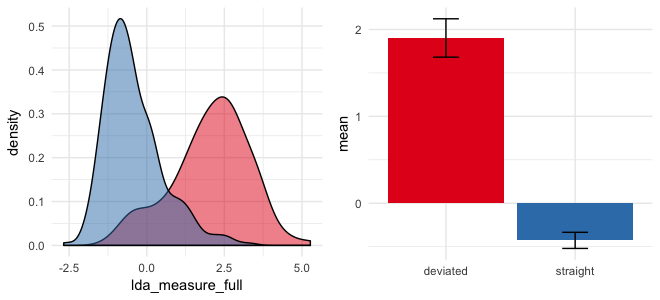
\includegraphics[width=\textwidth]{ldafull.png}
\caption{Coordinates, deltas and deltas-deltas as predictors}
\end{subfigure}
\begin{subfigure}{0.3\textwidth}
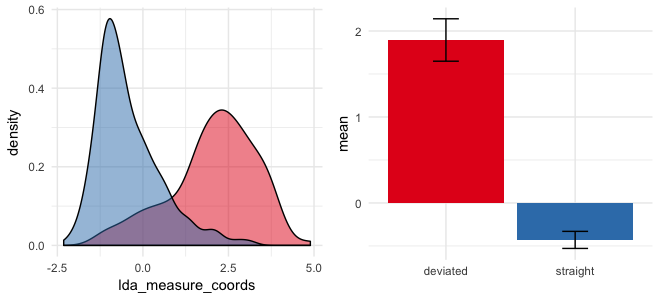
\includegraphics[width=\textwidth]{ldacoords.png}
\caption{Coordinates as predictors}
\end{subfigure}
\begin{subfigure}{0.3\textwidth}
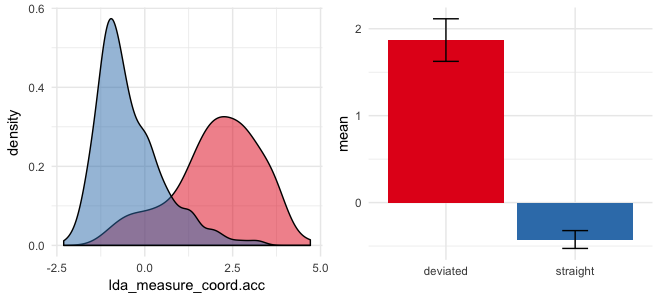
\includegraphics[width=\textwidth]{ldacoordsacc.png}
\caption{Coordinates and acceleration based on distance as predictors}
\end{subfigure}

\begin{subfigure}{0.3\textwidth}
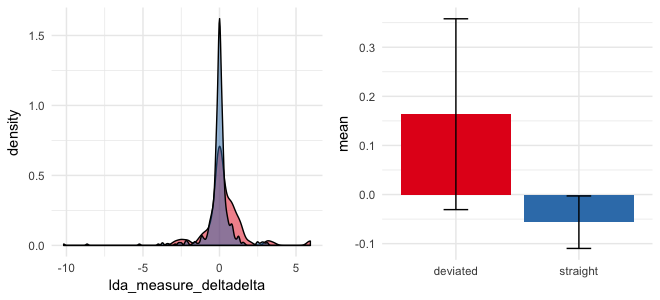
\includegraphics[width=\textwidth]{lda_deltadelta.png}
\caption{Deltas-Deltas as predictor}
\end{subfigure}
\begin{subfigure}{0.3\textwidth}
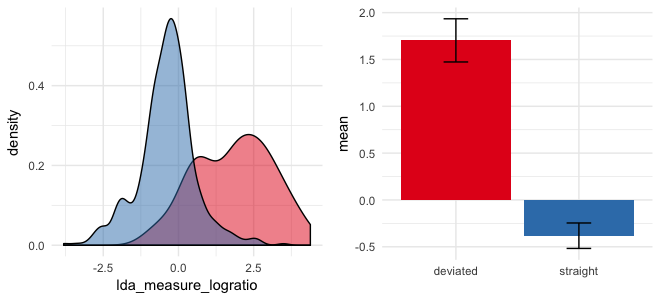
\includegraphics[width=\textwidth]{lda_logratio.png}
\caption{Log-ratios as predictor}
\end{subfigure}
\caption{Distribution and means}
\end{figure}



\begin{figure}[h]
\begin{subfigure}{0.3\textwidth}
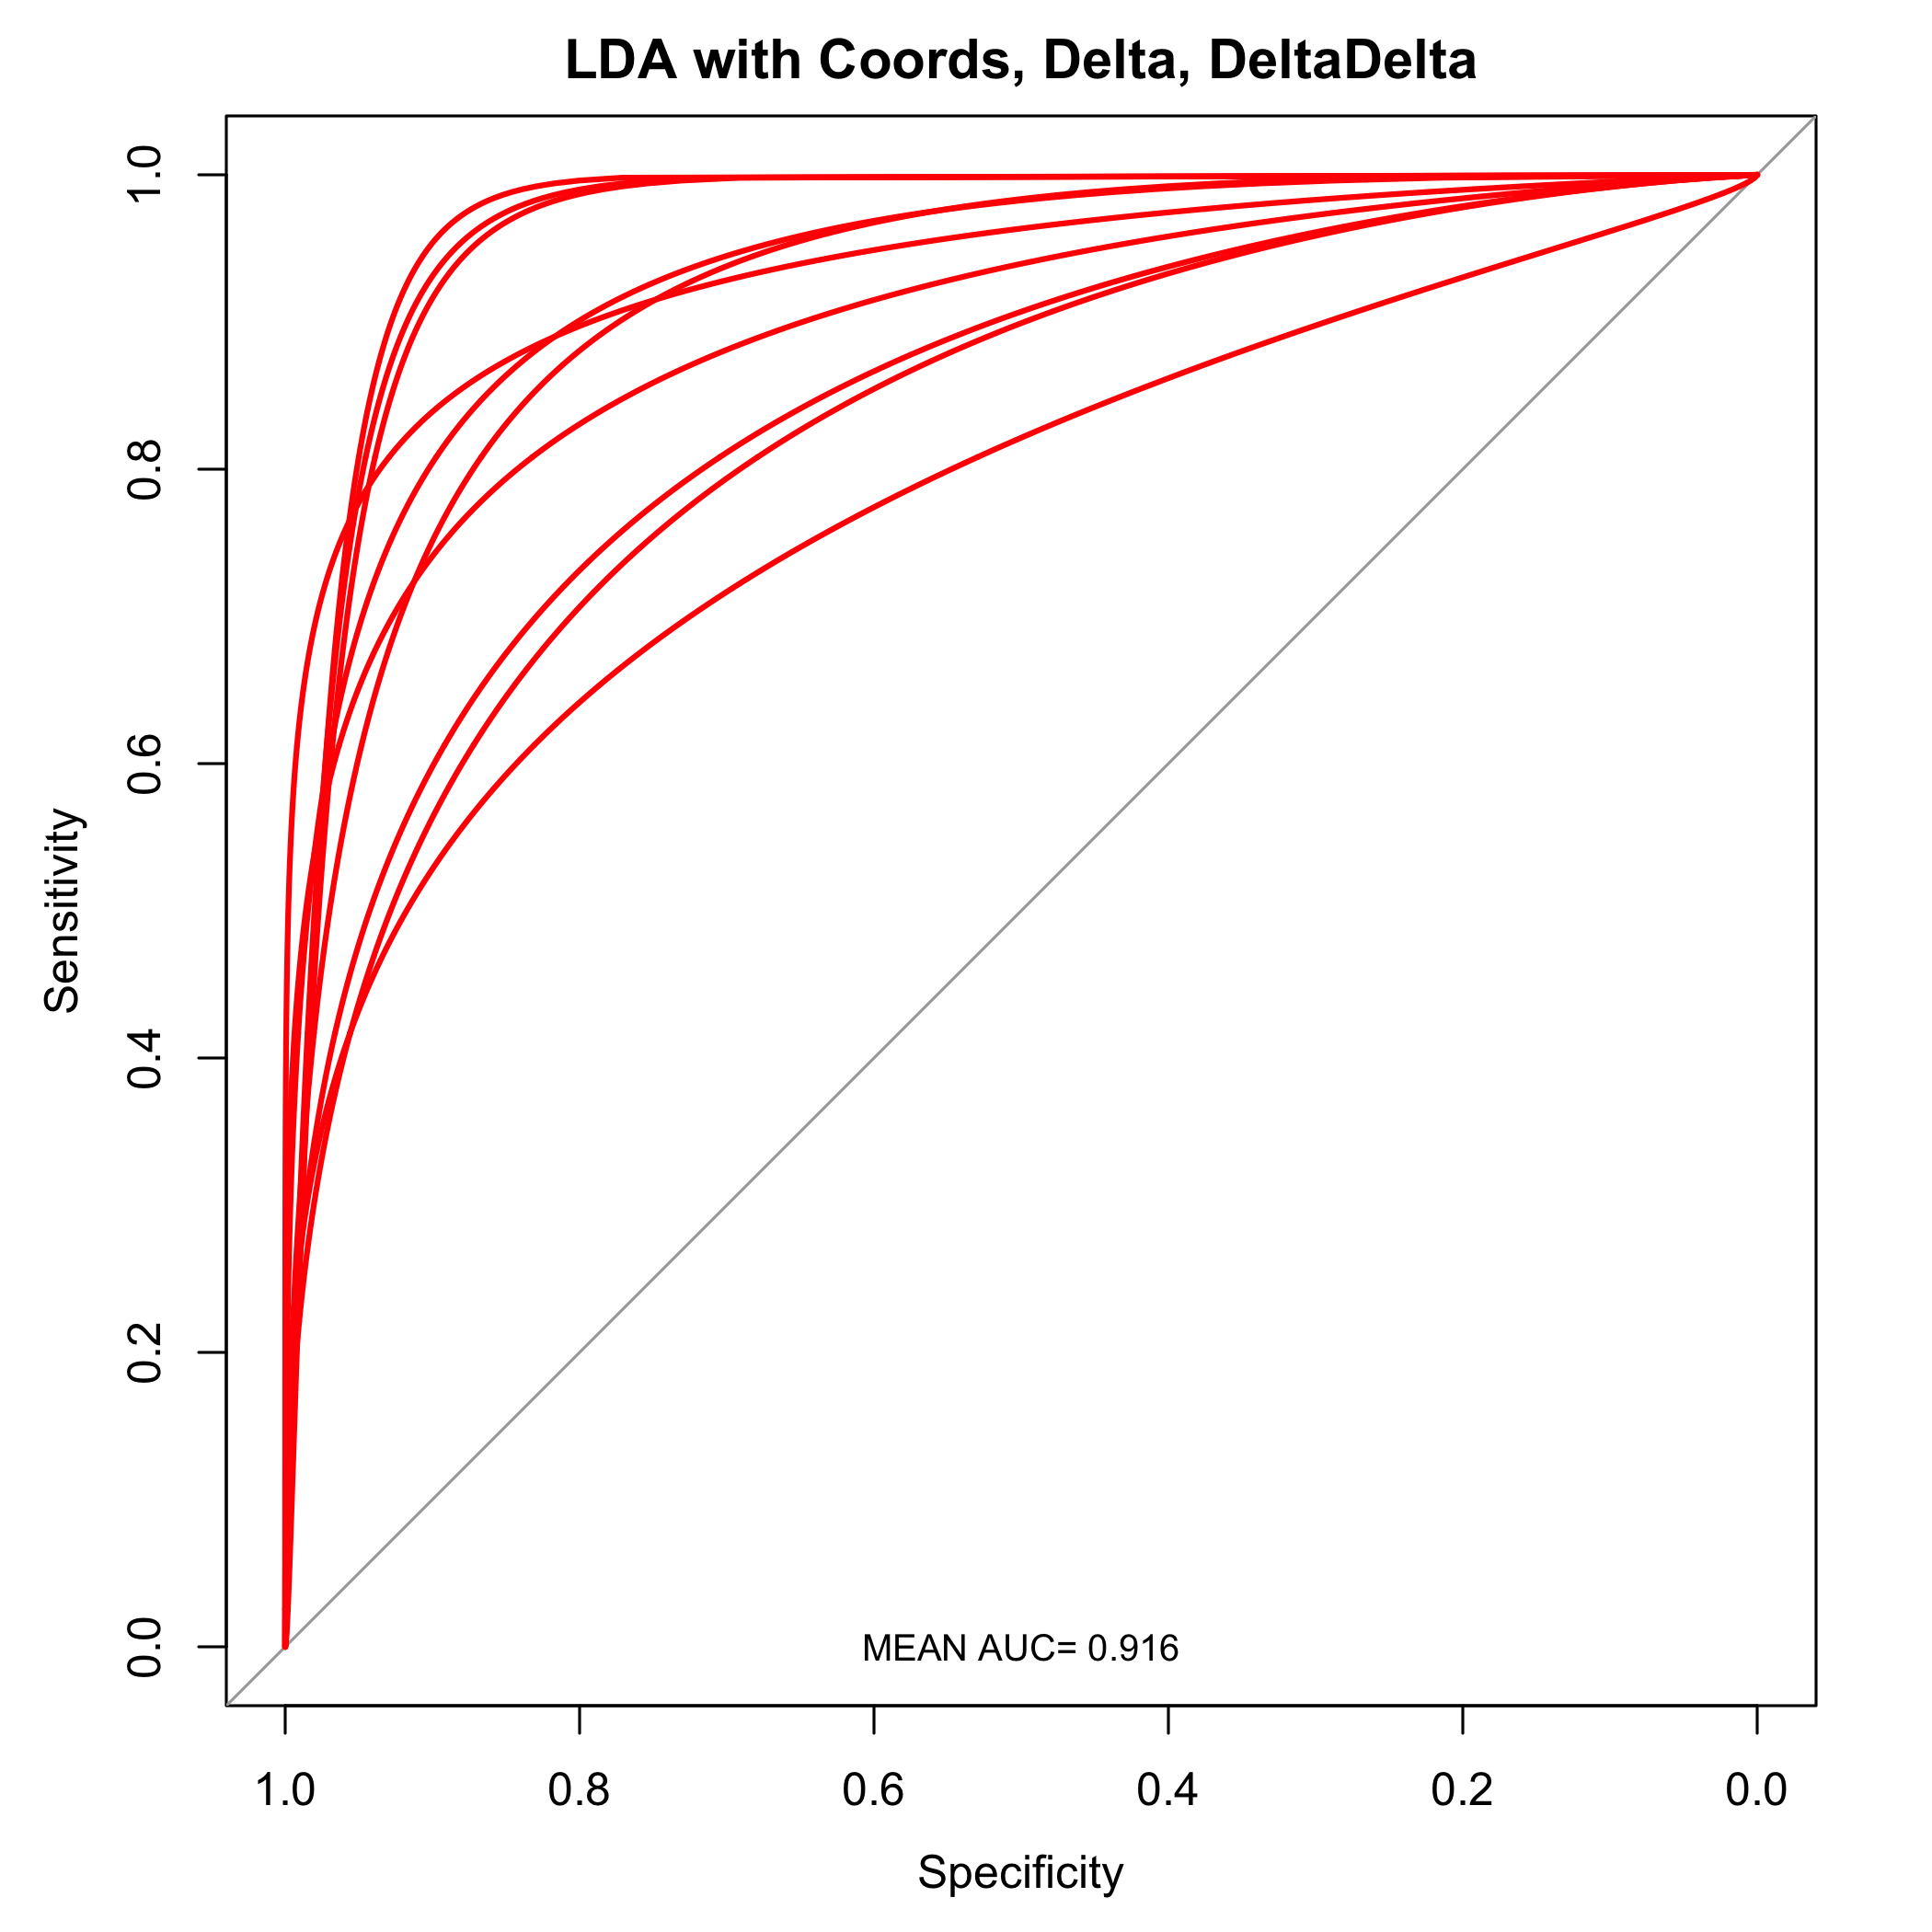
\includegraphics[width=\textwidth]{ROC_LDA-FULL.png}
\caption{Coordinates, deltas and deltas-deltas as predictors}
\end{subfigure}
\begin{subfigure}{0.3\textwidth}
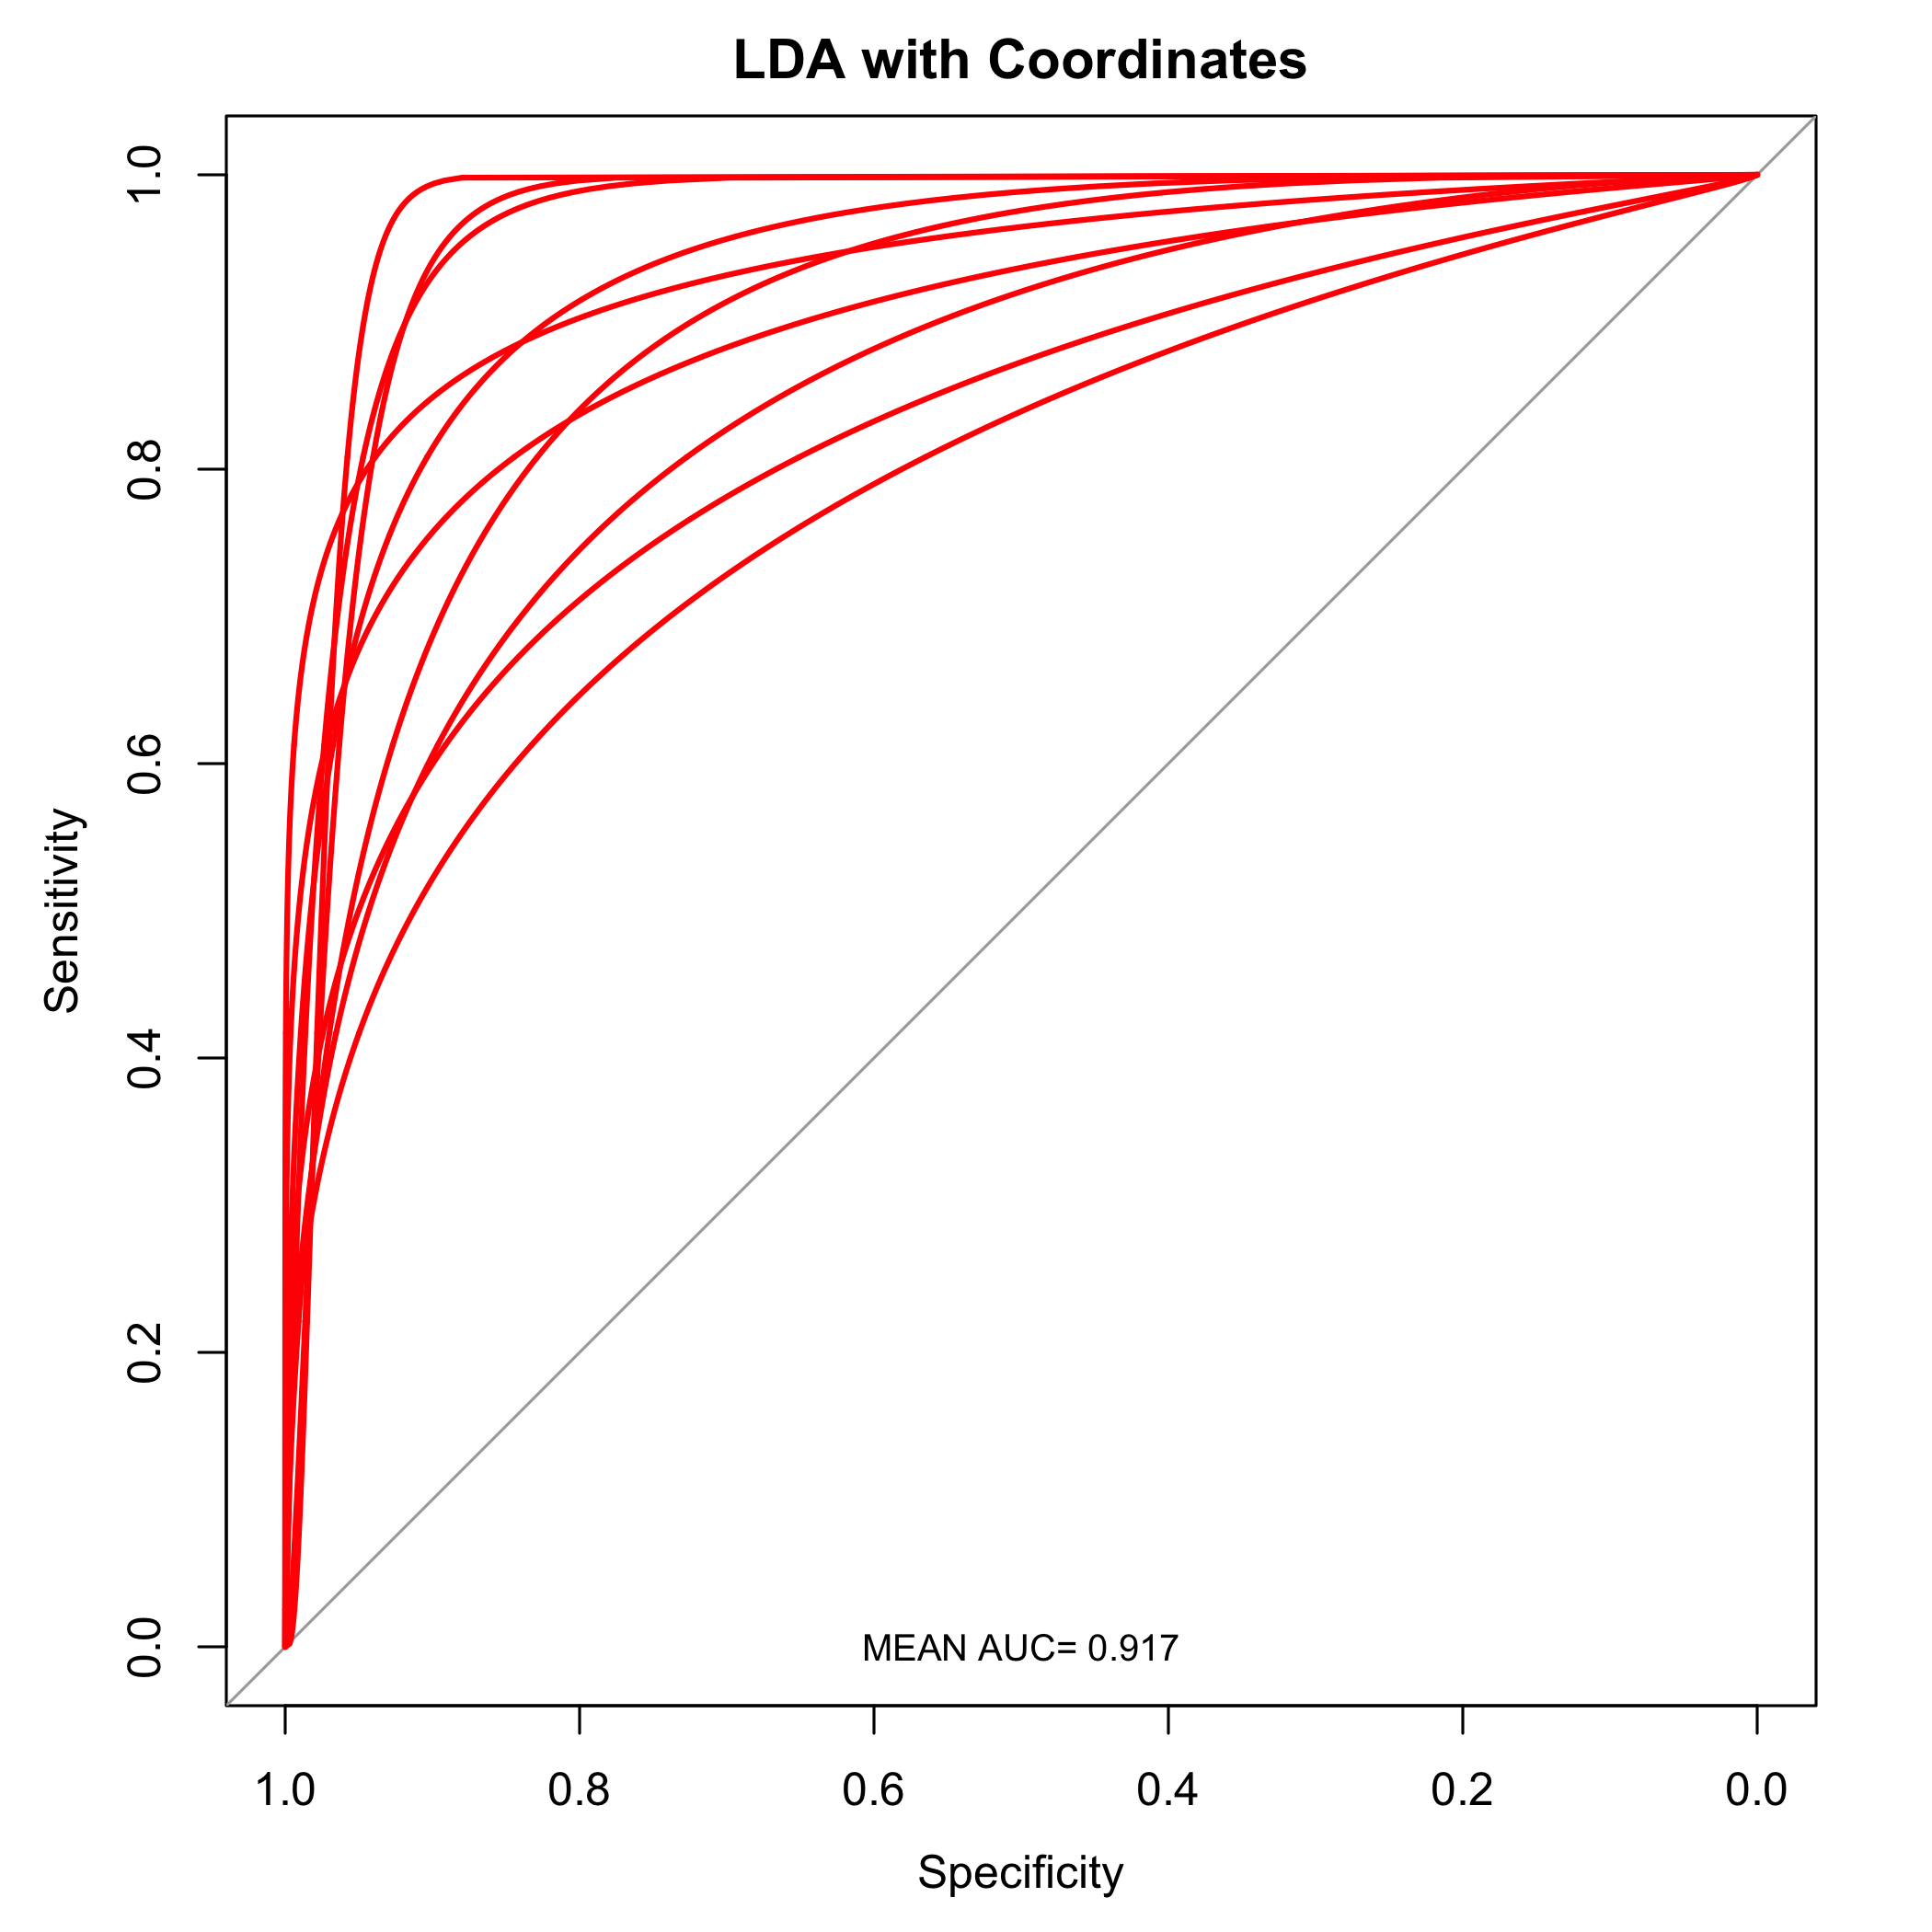
\includegraphics[width=\textwidth]{ROC_LDA-Coords.png}
\caption{Coordinates as predictors}
\end{subfigure}
\begin{subfigure}{0.3\textwidth}
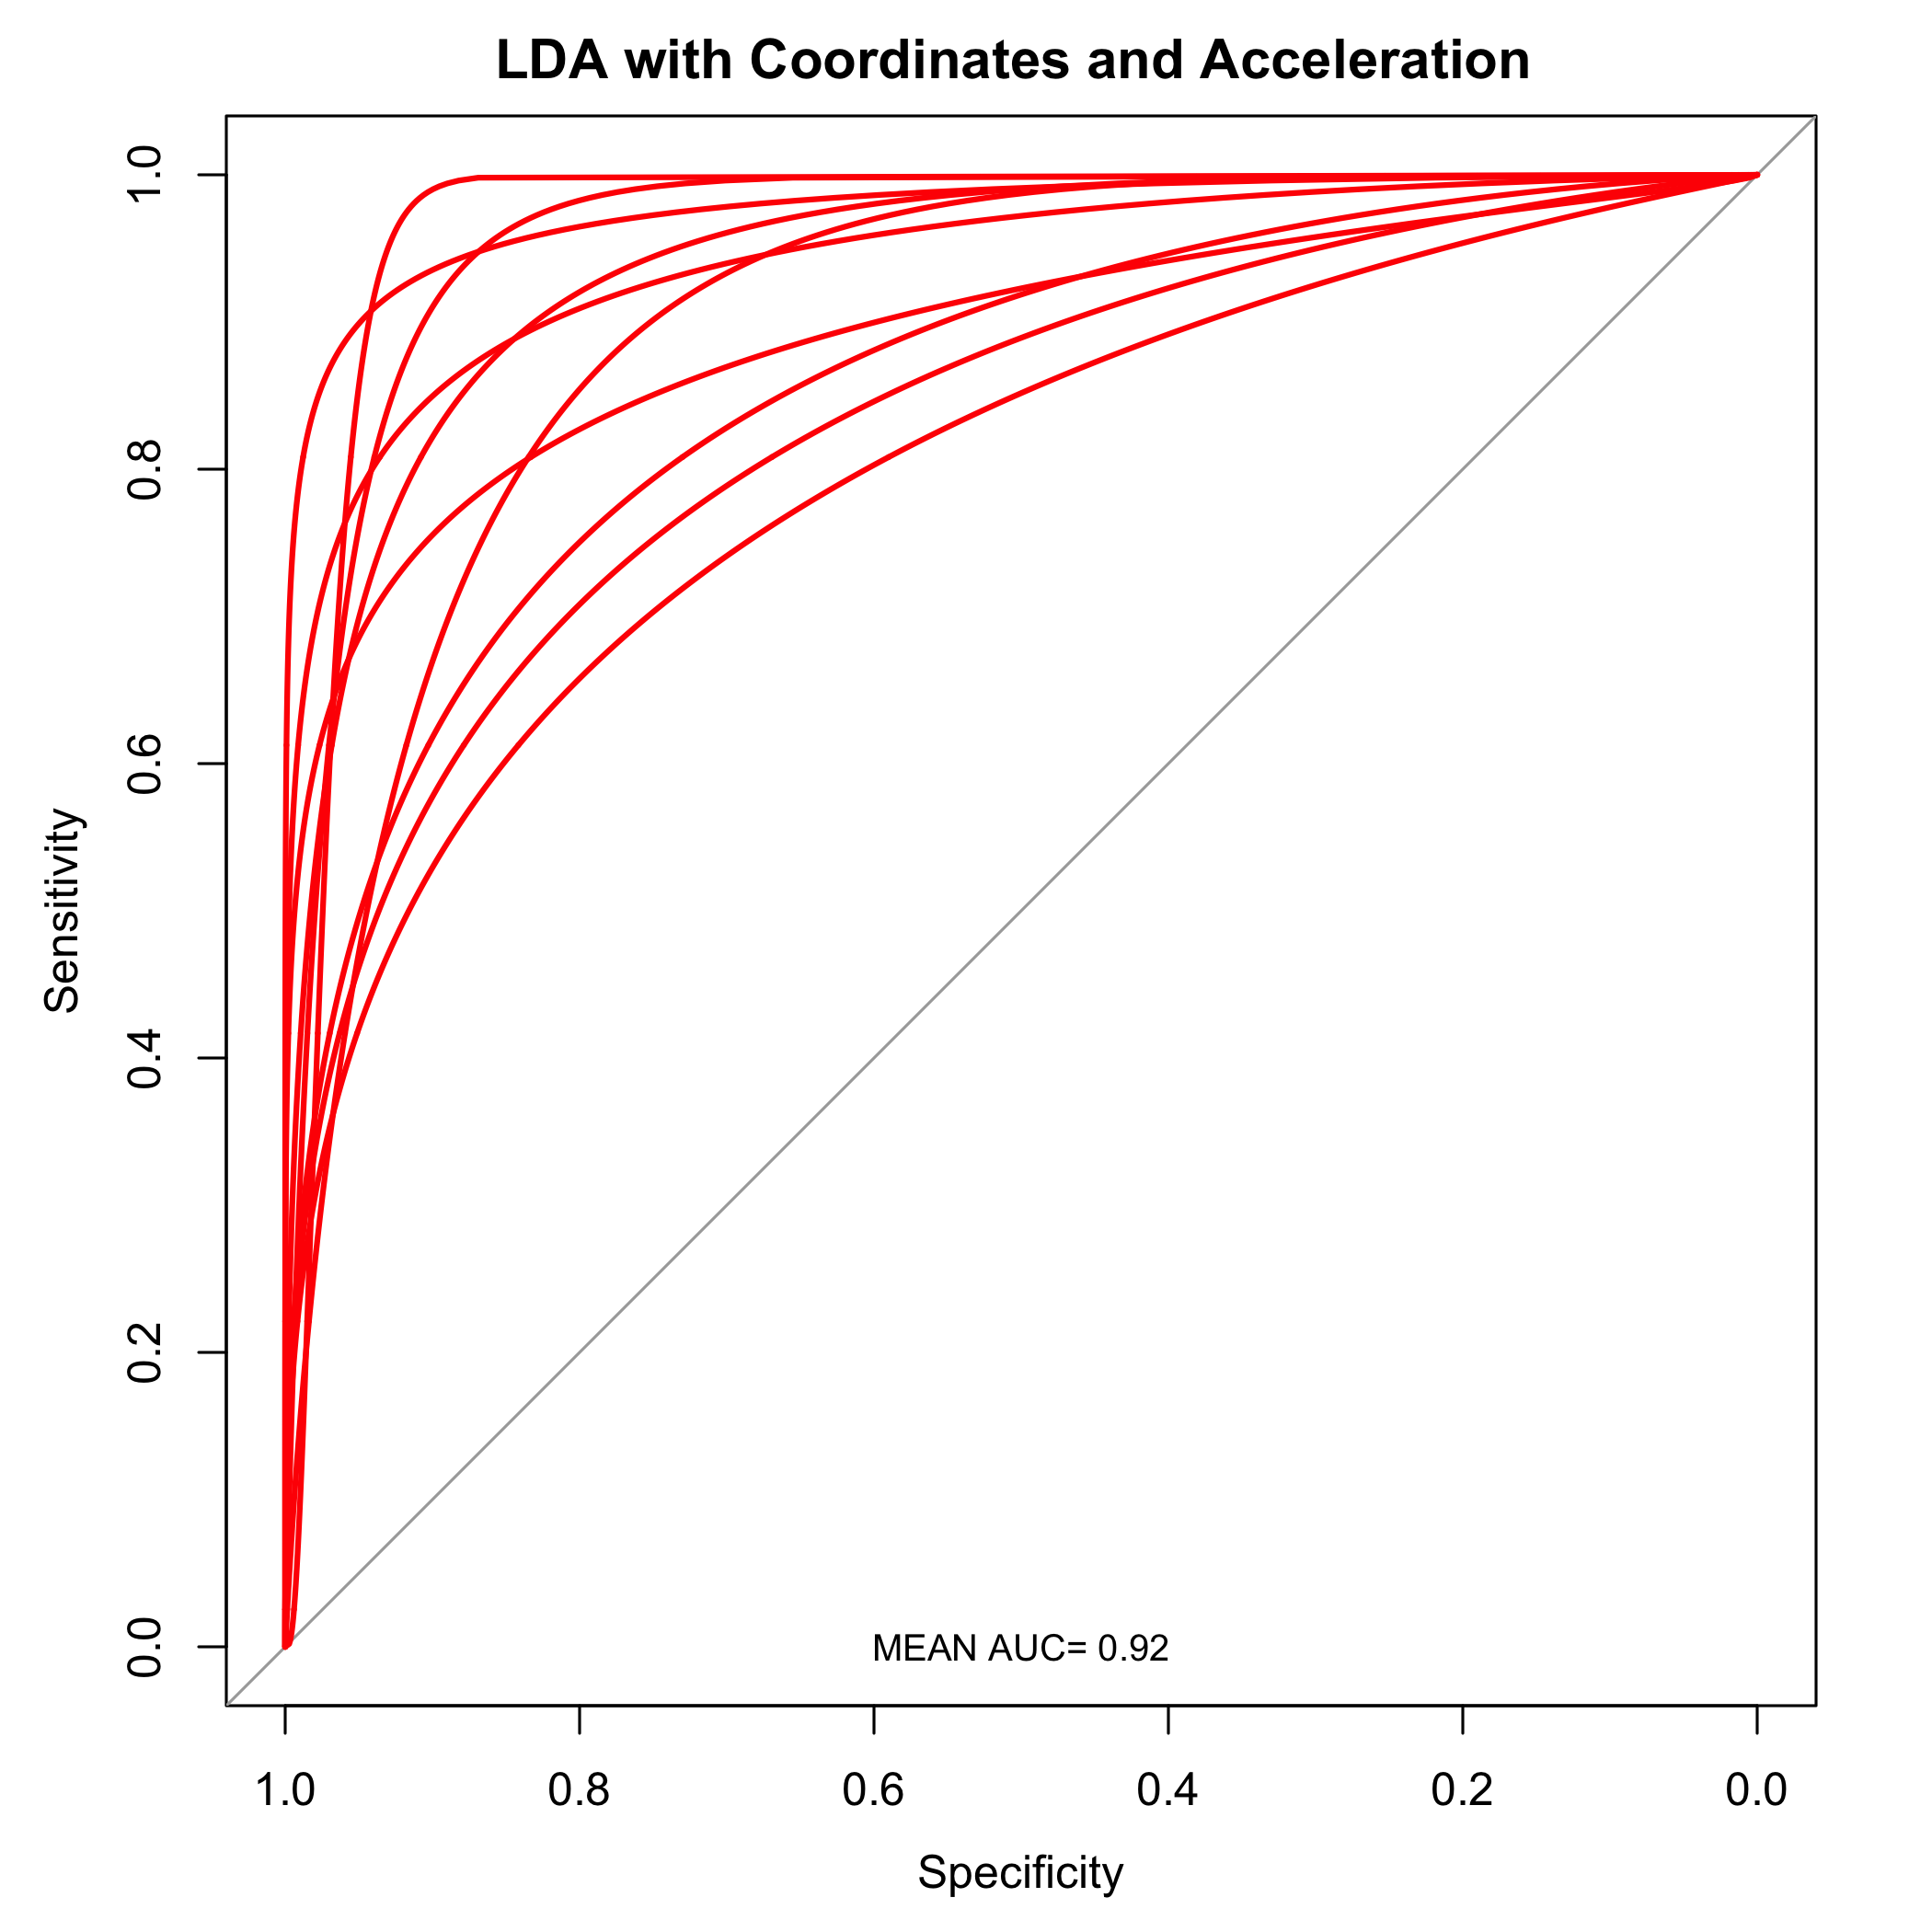
\includegraphics[width=\textwidth]{ROC_LDA-CoordsAcc.png}
\caption{Coordinates and acceleration based on distance as predictors}
\end{subfigure}

\begin{subfigure}{0.3\textwidth}
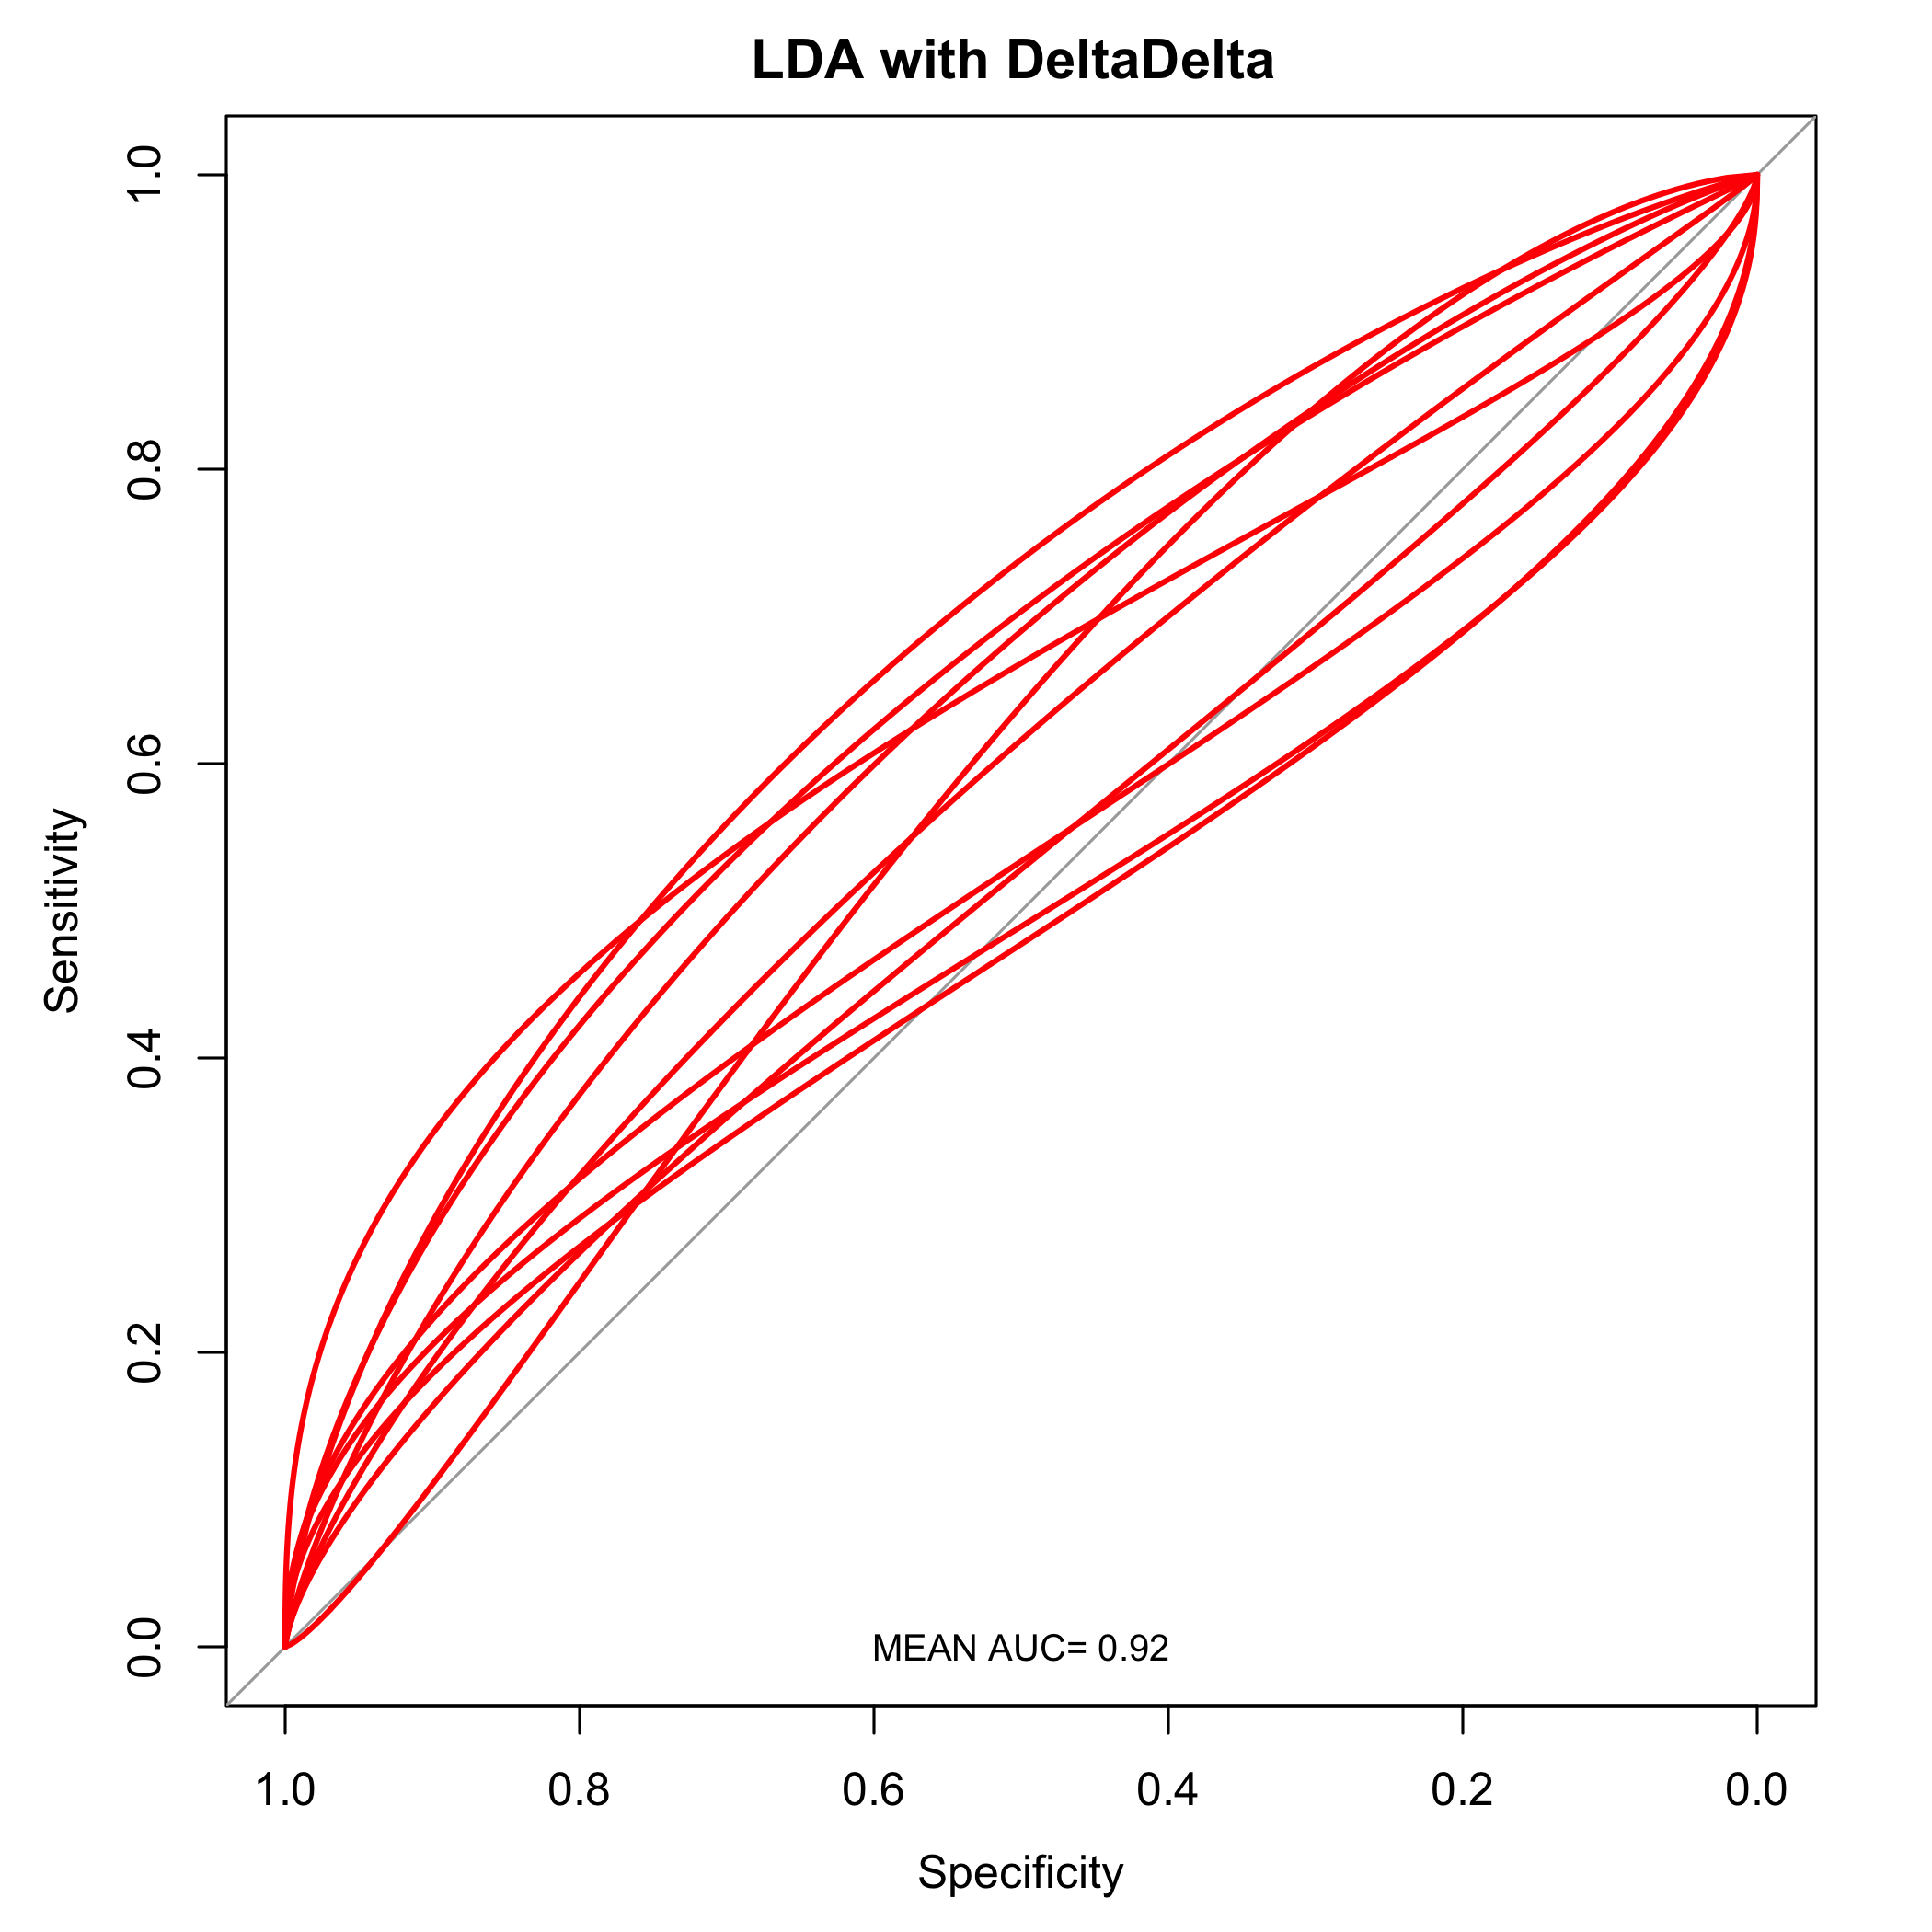
\includegraphics[width=\textwidth]{ROC_LDA-DeltaDelta.png}
\caption{Deltas-Deltas as predictor}
\end{subfigure}
\begin{subfigure}{0.3\textwidth}
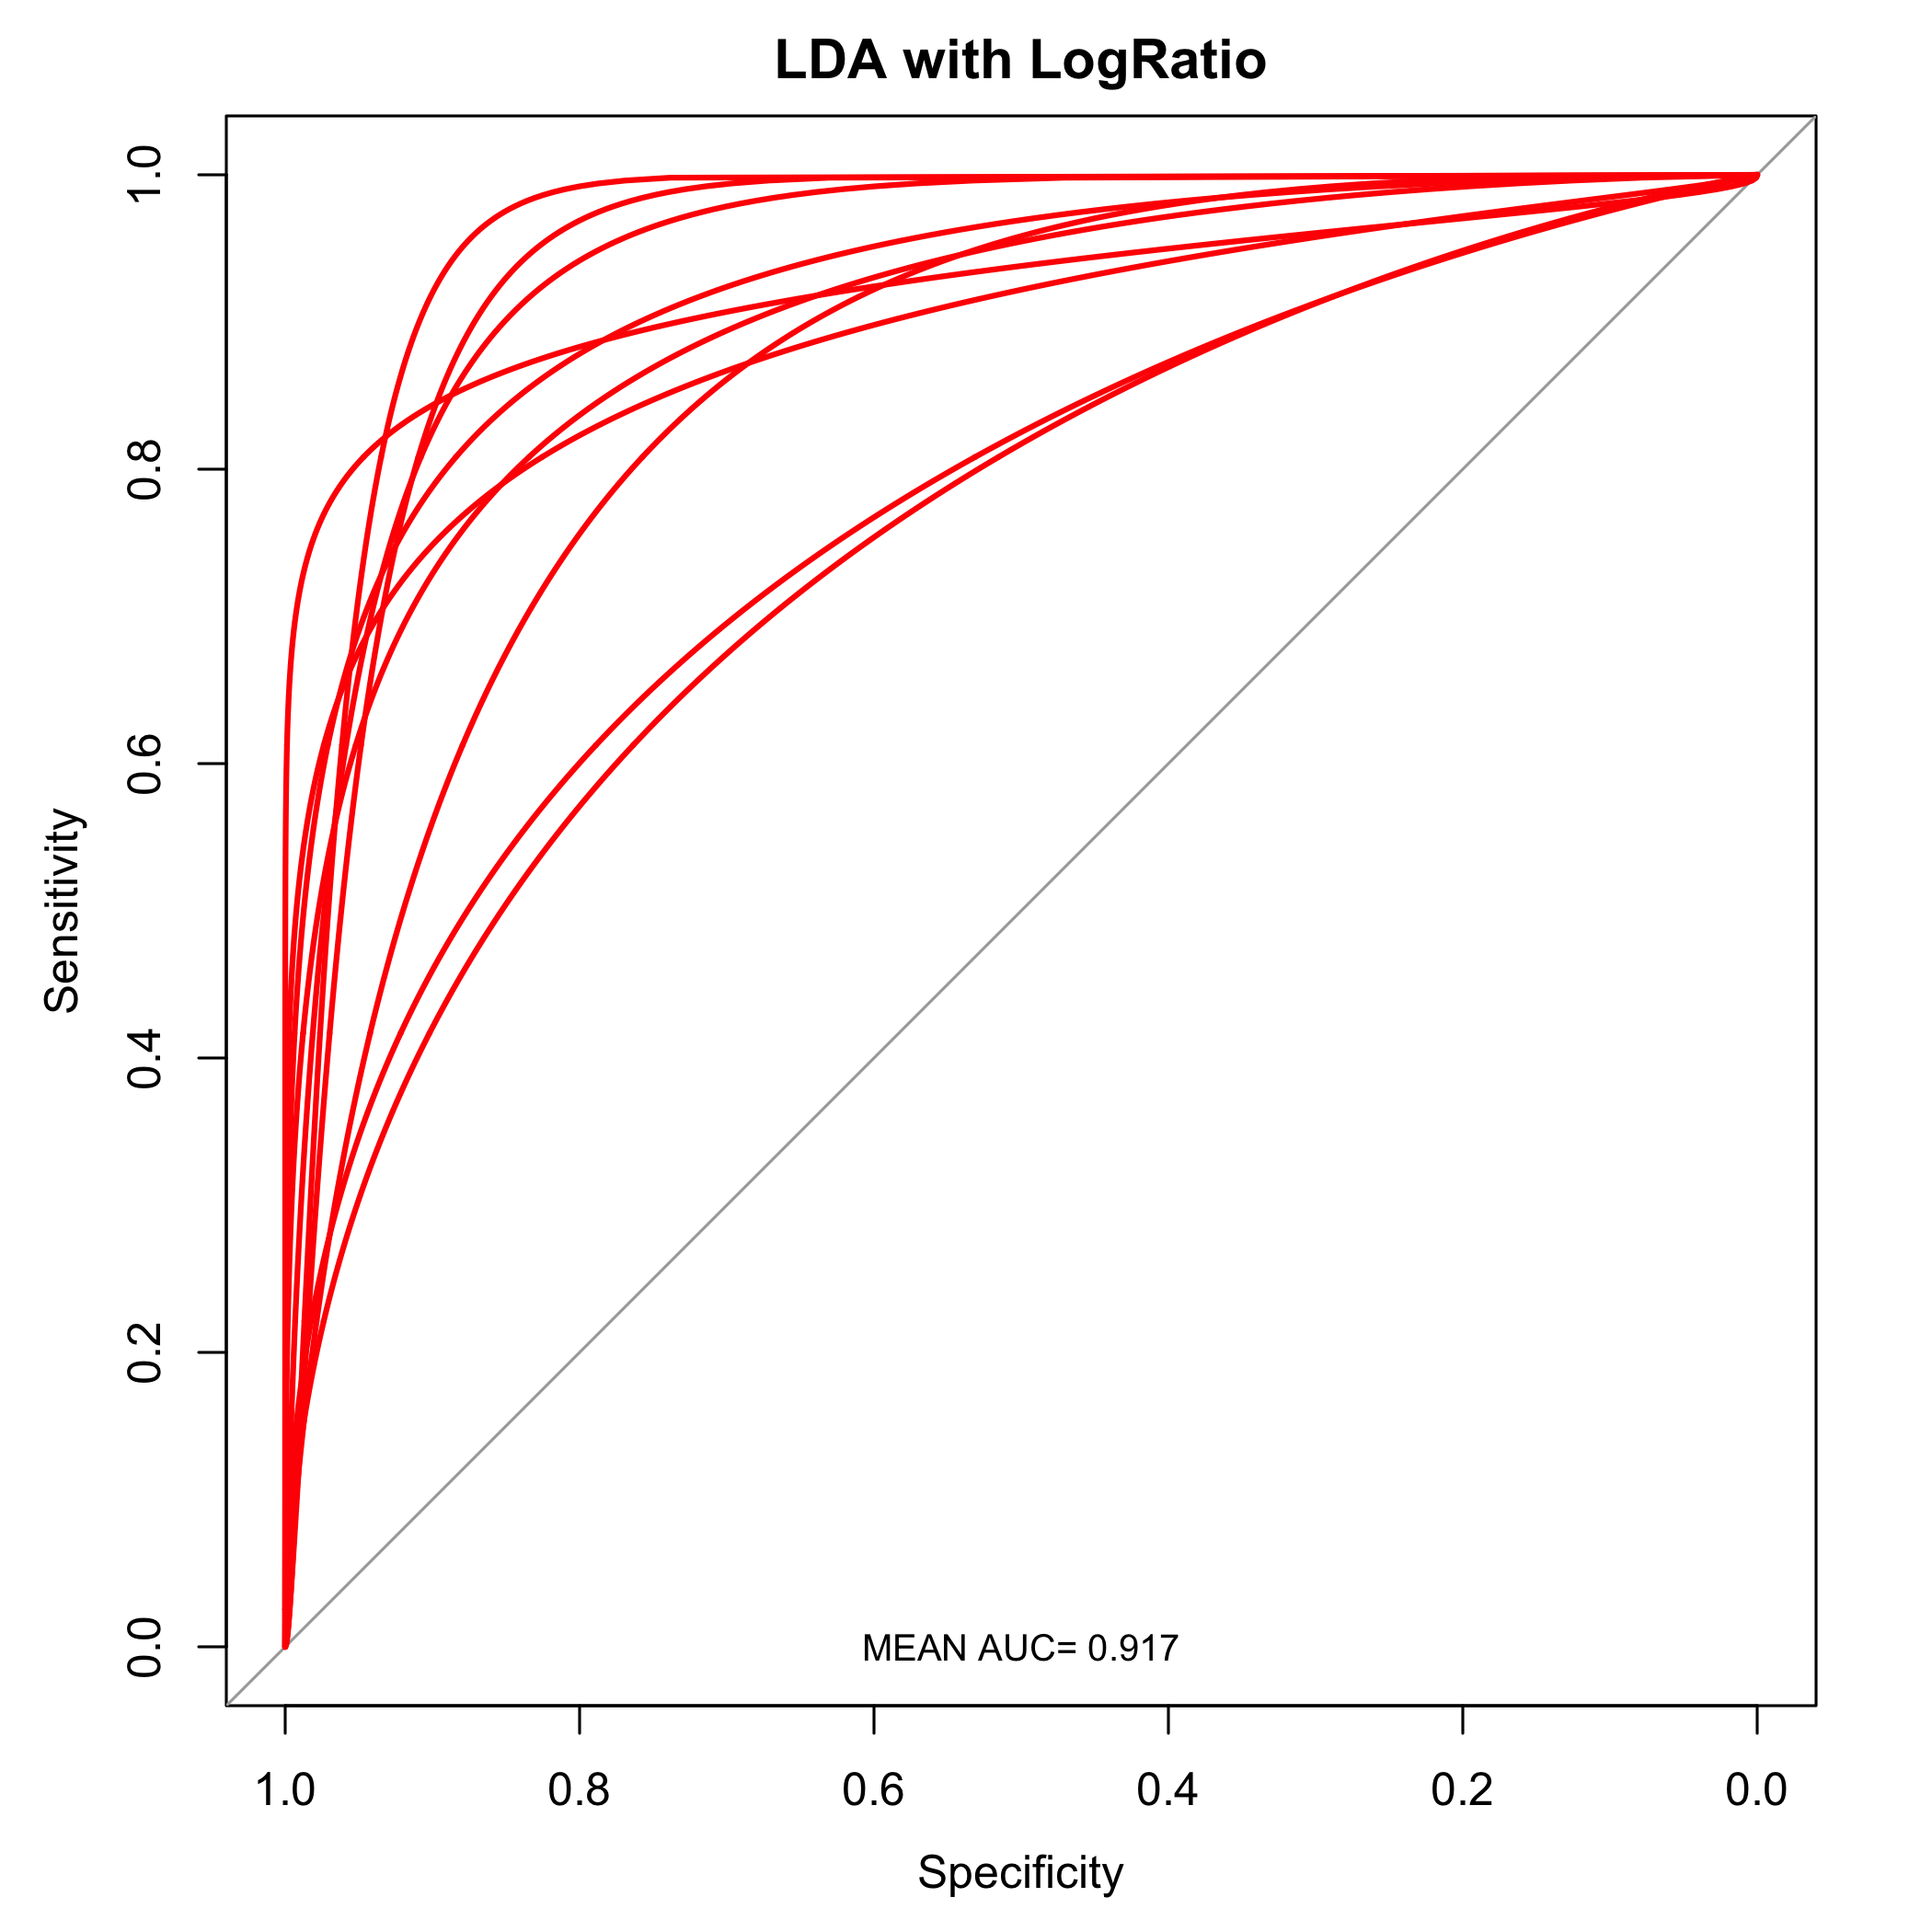
\includegraphics[width=\textwidth]{ROC_LDA-LogRatio.png}
\caption{Log-ratios as predictor}
\end{subfigure}
\caption{ROC and Area under the curve}
\end{figure}



\item[(B)] LDA vs. other measures (the ones reviewed in Section 1.2)

\begin{itemize}
\item Means and Distributions
\item Correlation matrix
\item AUC of ROC
\end{itemize}
\end{itemize}




\subsection{Discussion}

\begin{itemize}
\item Speed and acceleration do not seem to be good predictors of the difference between trajectories that underly more than one decision point and trajectories that underly only one decision point. This could be due to the specifics of our data, which is very noisy (online experiment).

\item Both the LDA classifier and more traditional measures suggest that \emph{spatial} components, such as \textit{x,y} coordinates, are informative about the underlying decision processes (and also robust to noise). 

\item Decision about the different LDAs?

\item Note about the experiment itself: Does this validation experiment really mimic decision taking? 

\end{itemize}


\section{Testing the classifier on negation data}
\addMM{MM: Are we going to test all LDAs with the negation data, or only the one that gives best results above? (Note that we already know that most LDAs are equivalent to each other.)}
\begin{itemize}

\item Given the good performance of our classifier with controlled/validation data, we can now 
apply it to new data. We aim to replicate D\&D results for negation and test them with our classifier.

\item We expect that our classifier (trained with validation data) will success in dissociating trials involving negative and positive sentences. If this is the case, we will be providing additional support to the hypothesis that negation involves a two-step derivation (i.e. an unconscious change of decision). 

\item It should be noticed, however, that the calibration data is only an approximation of what should happen in an unconscious change of decision, such as the one expected for negation processing.


\end{itemize}

 


\subsection{Replication Dale and Duran 2011}

\begin{table}[h]
\centering
\begin{tabular}{ccc}
Truth value & Polarity & Example \\
\hline
\multirow{2}{*}{True} & Positive & Cars have wheels.\\ 
 & Negatives & Cars have no wings.\\ 
\hline
\multirow{2}{*}{False} & Positive & Cars have wings.\\ 
 & Negatives & Cars have no wheels.\\
\end{tabular}
\caption{Design}
\end{table}

\subsection{Results}

\begin{itemize}
\item Performance (compare with Dale and Duran)
\item Descriptive statistics?
\item Performance of the classifier trained above
\item Performance of other measures
\end{itemize}








\end{document}
